The PFEM-2 method is a generalization of the Particle Finite Element Method (PFEM) \cite{sergio:pfem} where the particles are not restricted to the mesh nodes. Massless particles are added everywhere in the mesh and the advection is done by transporting the particles. The main benefit is that now the nodes of the mesh do not have to be moved as was the case in \cite{sergio:pfem} saving many re-meshing operations while maintaining the Lagrangian advection. In \cite{sergio:xivs1} Idelsohn et al. present an integration scheme called {\em eXplicit Integration following the Velocity Streamlines} (X-IVS) which is used to integrate the trajectory of particles in PFEM-2. Using this technique the position of a particle $p$ at time $t^n$ ($x_p^{n+1})$ is computed using the velocity streamlines at $t^n$:

\begin{equation}\label{xivs}
  \begin{cases}
    x_p^{n+1}=x_p^n+\int_n^{n+1} u^n(x_p^\tau) d\tau\\
    \hat{u}^{n+1}_p=u_p^n
  \end{cases}
\end{equation}

The expresion in eq. \ref{xivs} is explicit since it only depends on values from time step $t^n$ maintaing the high order approximation used for the velocity field. This expresion is not and exact integration since the integral is evaluated following a pseudo-trajectory of the particles calculated with the velocity streamlines within each time step instead of following the true trajectory. Eq \ref{xivs} may be integrated analytically or using any standard time integration scheme like explicit Runge-Kutta or using sub-stepping. This new integration proposal provides an efficient strategy to emply time-steps which allow a Courant-Friedrich-Levy (CFL) number larger than one, being:
\begin{equation}
  CFL=\frac{|\vect{u}|\Delta t}{\Delta x}
\end{equation}
In summary  this means that each particle will be able to travel more than one element without compromising the stability of the method.

\begin{figure}[htp] 
\centering 
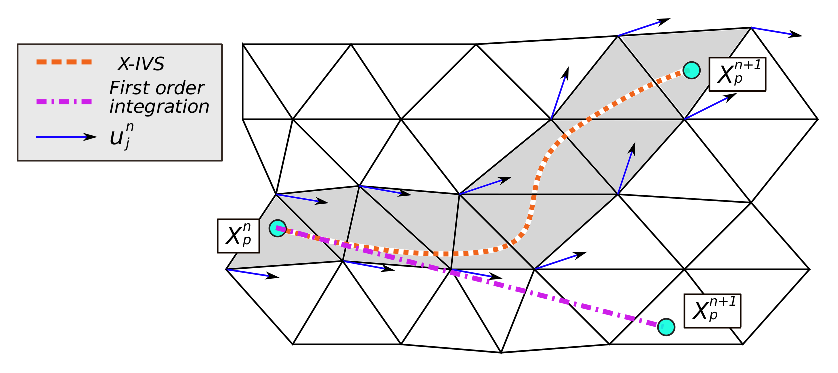
\includegraphics[scale=.8]{./imgs/xivs.eps}
\caption{Comparison of the trajectory of a particle moving from $x_p^n$ to $x_p^{n+1}$ for a given $\Delta t$ using the X-IVS method and a first order integration method. The vecotrs represent the fluid velocity at time $t^n$.}
\label{fig:xivs}
\end{figure}

In figure \ref{fig:xivs} the trajectory of a particle is computed using the X-IVS method and it is compared to the trajectory of a first order integration scheme for a $CFL>1$. 
